\documentclass[UTF8]{ctexart}
\usepackage{graphicx}
\usepackage{subfigure}
\usepackage{float}
\usepackage{geometry}

\geometry{left=2.0cm, right=2.0cm, top=2.5cm, bottom=2.5cm}
\title{第一次技术文档}
\author{刘畅 15061183}

\begin{document}
	\maketitle
	% \tableofcontents
	\section{程序说明}
	\noindent
	\textbf{使用语言:} JAVA \newline
	\textbf{编程环境:} Windows 8.1 + Eclipse Neon.3 Release (4.6.3) \newline
	\textbf{主要方法:} \newline
	\begin{tabular}{p{10cm}p{7cm}}
	\hline
	\textbf{方法名}& \textbf{作用} \\
	\hline
	void grayscale(String outputLabel) {..}&  生成灰度图\\
	\hline
	void globalStretch(String outputLabel, int lowerScale, int upperScale) {..}&  提供变化后的灰度范围,对灰度图进行全局线性拉伸(压缩)\\
	\hline
	void localStretch(String outputLabel, int oriLowerScale, int oriUpperScale, int lowerScale, int upperScale) {..}&  提供原灰度图灰度范围和变化后的灰度范围,对灰度图进行局部线性拉伸,可能改变图片整体灰度范围\\
	\hline
	void piecewiseStretch(String outputLabel, int oriLowerScale, int oriUpperScale, int lowerScale, int upperScale) {..}& 提供原灰度图灰度范围和变化后的灰度范围,对灰度图进行局部线性拉伸,不会改变图片整体灰度范围 \\
	\hline
	void histogramCorrection(String outputLabel, int partNum) {..}&  给定分段数,对灰度图进行直方图均衡处理\\
	\hline
	\end{tabular}

	\section{准备工作:图片灰度化}
		\subsection{实现过程}
			\subsubsection{灰度矩阵的获取}
			在对一个宽度为$w$、高度为$h$图片进行\textbf{直方图均衡}和\textbf{灰度线性拉伸}处理之前,需要先对图像进行灰度化处理。假设某像素灰度级为$Y$,根据像素的$R$、$G$、$B$值利用公式
			\[ Y=0.3R+0.59G+0.11B \]
			将每个点的灰度级$Y$记录在灰度矩阵$M(w,h)$中。
			\subsubsection{输出灰度图}
			根据灰度矩阵$M(w,h)$,建立一个宽度为$w$,高度为$h$的新图片,并将图片上任意一个像素点的$R$、$G$、$B$值都设定为$M(w,h)$中对应位置的灰度级$Y$,保证图片各个像素点$R$、$G$、$B$值相等。该图即为原图的灰度图。
		\subsection{处理效果}

		\begin{figure}[H]
		\centering
		\subfigure[原彩色图]{
			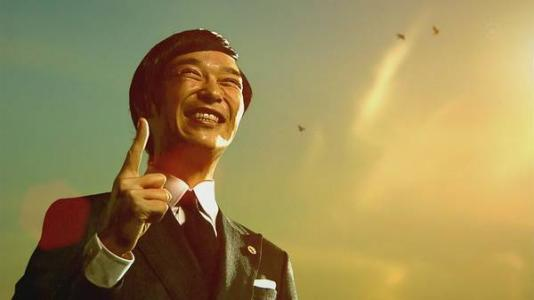
\includegraphics[width=0.4\textwidth]{lh_color.jpg}}
		\subfigure[处理后灰度图]{
			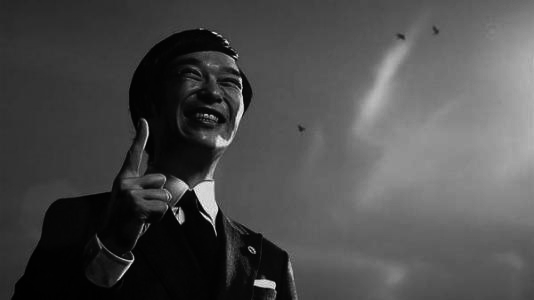
\includegraphics[width=0.4\textwidth]{lh_grey.png}}
		\caption{灰度处理效果}
		\end{figure}


	\section{任务一:直方图均衡}
		\subsection{算法实现}
		根据读取图像得到的灰度矩阵$M(w,h)$,可以计算出第$i$种灰度所占的像素数量$n_i$。假设灰度级为$L$(在该程序中,取$L=256$),则第$k$个灰度级均衡变换后的新灰度级$s_k$可由以下公式得到:
		\[ s_k=(L-1)\sum_{i=0}^k\frac{n_i}{wh} \]

		\subsection{处理效果}
			\subsubsection{图片一}
			\begin{figure}[H]
			\centering
			\subfigure[原灰度图]{
				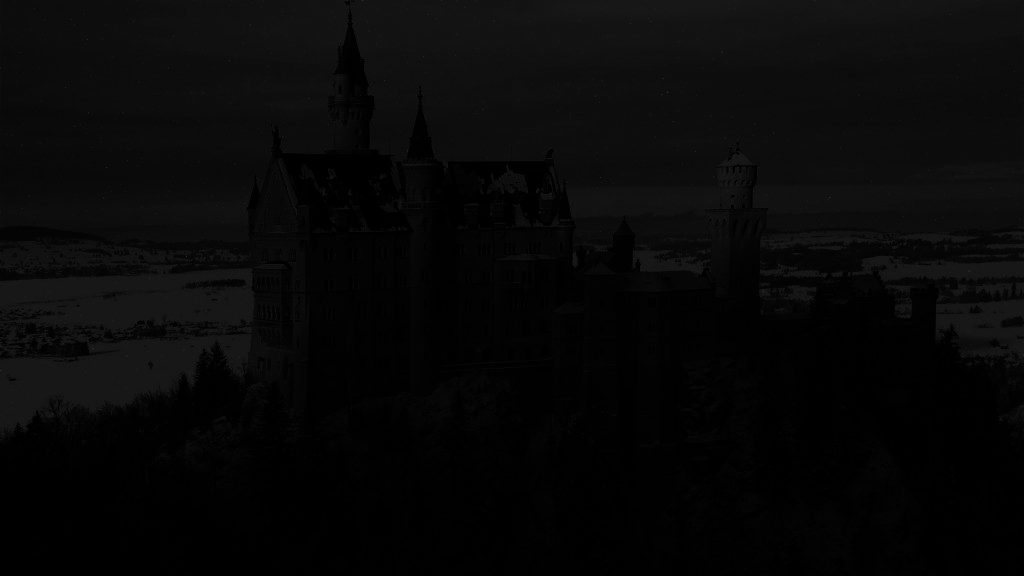
\includegraphics[width=0.4\textwidth]{cas_grey.png}}
			\subfigure[均衡处理后灰度图]{
				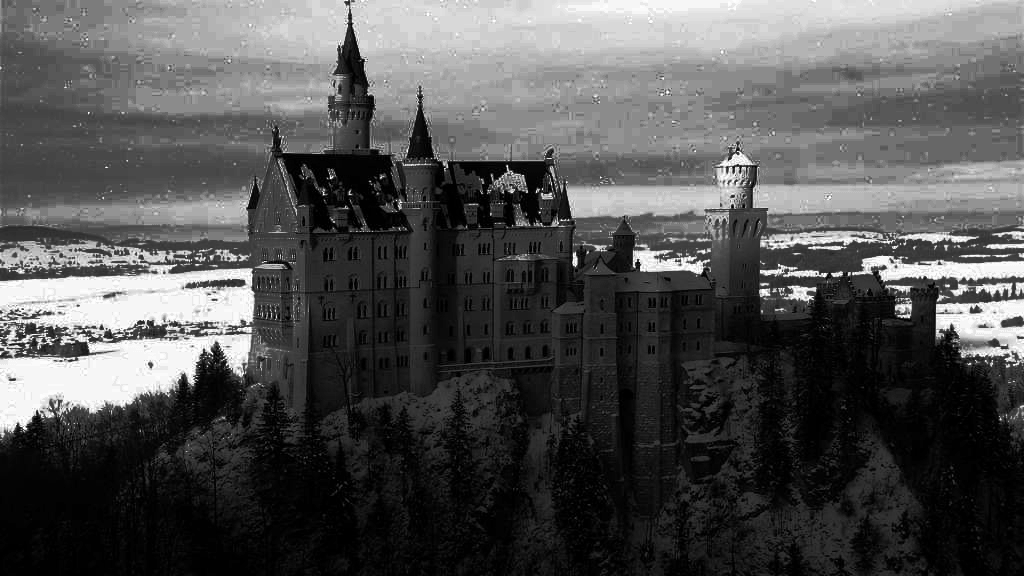
\includegraphics[width=0.4\textwidth]{cas_cor_1.png}}
			\subfigure[原灰度分布]{
				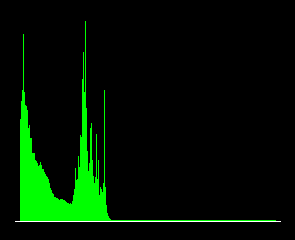
\includegraphics[width=0.4\textwidth]{cas_grey_hist.png}}
			\subfigure[均衡处理后灰度分布]{
				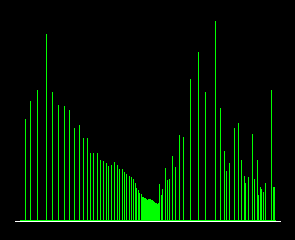
\includegraphics[width=0.4\textwidth]{cas_cor_1_hist.png}}
				\caption{图片二直方图均衡效果}
			\end{figure}

			可以看到,整体偏暗的城堡画面经过直方图均衡处理后变得清晰许多,直方图也的确变得更分散了,这符合算法的预期。

			\subsubsection{图片二}
			\begin{figure}[H]
			\centering
			\subfigure[原灰度图]{
				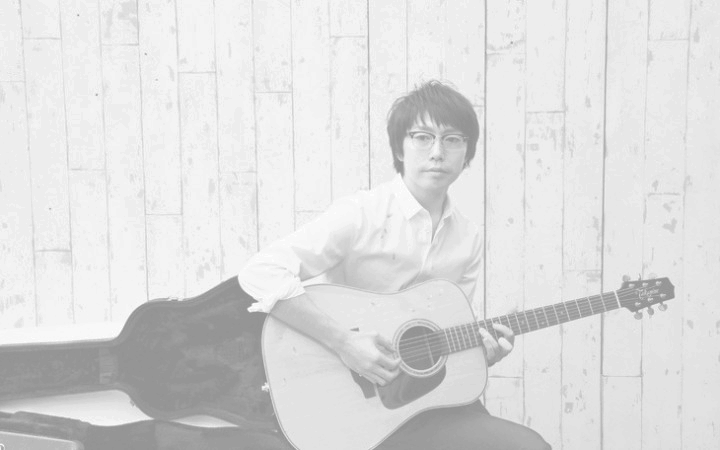
\includegraphics[width=0.4\textwidth]{yuu_grey.png}}
			\subfigure[均衡处理后灰度图]{
				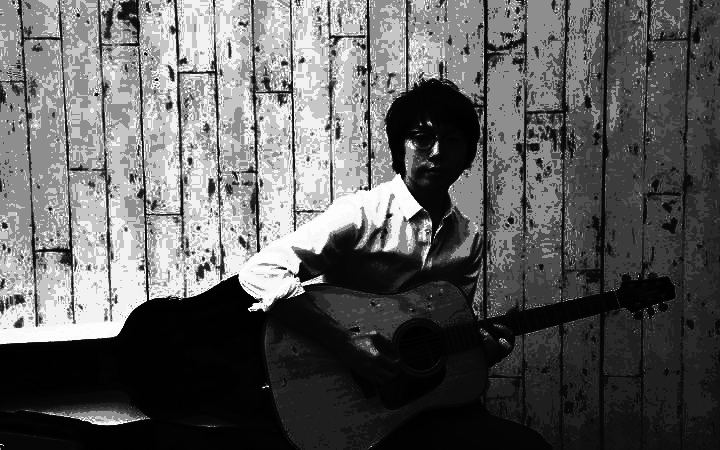
\includegraphics[width=0.4\textwidth]{yuu_cor_1.png}}
			\subfigure[原灰度分布]{
				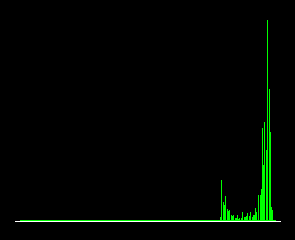
\includegraphics[width=0.4\textwidth]{yuu_grey_hist.png}}
			\subfigure[均衡处理后灰度分布]{
				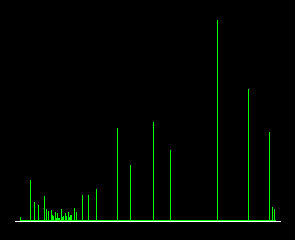
\includegraphics[width=0.4\textwidth]{yuu_cor_1_hist.png}}
				\caption{图片二直方图均衡效果}
			\end{figure}

			在图片二中,直方图均衡的结果虽然正确,但其效果并不理想,主要体现在均衡结果中人物部分的灰度级过高,以至于看不清具体细节。

			\subsubsection{图片三}
			\begin{figure}[H]
			\centering
			\subfigure[原灰度图]{
				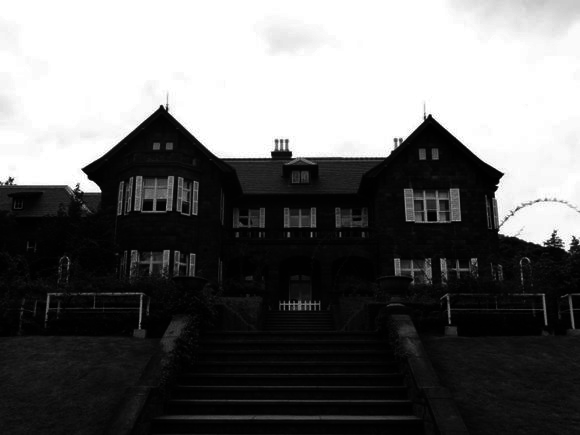
\includegraphics[width=0.4\textwidth]{rokkenjima_grey.png}}
			\subfigure[均衡处理后灰度图]{
				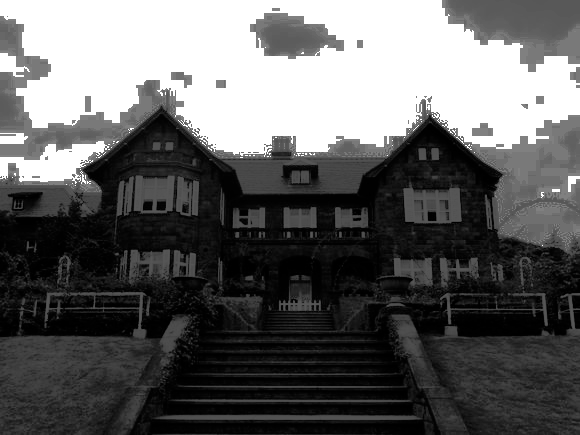
\includegraphics[width=0.4\textwidth]{rokkenjima_cor_1.png}}
			\subfigure[原灰度分布]{
				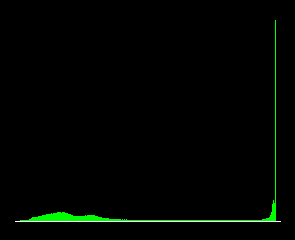
\includegraphics[width=0.4\textwidth]{rokkenjima_grey_hist.png}}
			\subfigure[均衡处理后灰度分布]{
				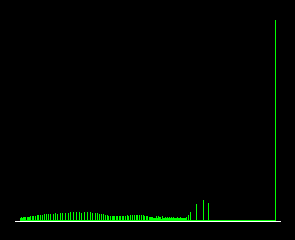
\includegraphics[width=0.4\textwidth]{rokkenjima_cor_1_hist.png}}
				\caption{图片三直方图均衡效果}
			\end{figure}

			在图片三中,天空部分出现了出现了不自然的像素块,效果也不是很理想。

		\subsection{改进}
			\subsubsection{算法}
			从图3中可以看到,效果不理想的主要原因是图片整体灰度级较低,而图片中人物的灰度级相较偏高,导致均衡后灰度级大大上升。为了解决大量低灰度对高灰度的干扰,我尝试将处理前的灰度级进行分段操作,如低灰度区和高灰度区,然后在这两部分分别进行直方图均衡处理,避免了低灰度区对高灰度区的干扰。\newline
			\indent 假设灰度的分段数为$p$,首先采用以下公式计算出平均每段的像素数$n_{avg}$:
			\[ n_{avg} = \frac{wh}{p} \]
			之后,根据$n_avg$对灰度级由低至高进行分段,尽可能保证每段内像素数总和相等。假设第$k$个灰度级所处段的最低灰度级为$r_{min}$,最高灰度级为$r_{max}$,则其均衡变换后的新灰度级$s_k$可由以下公式得到:
		\[ s_k=r_{min}+(r_{max}-r_{min})\sum_{i=r_{min}}^k\frac{n_i}{\sum_{j=r_{min}}^kn_j} \]


		 	\subsubsection{效果}
			\begin{figure}[H]
			\centering
			\subfigure[直方图均衡后灰度图(p=1)]{
				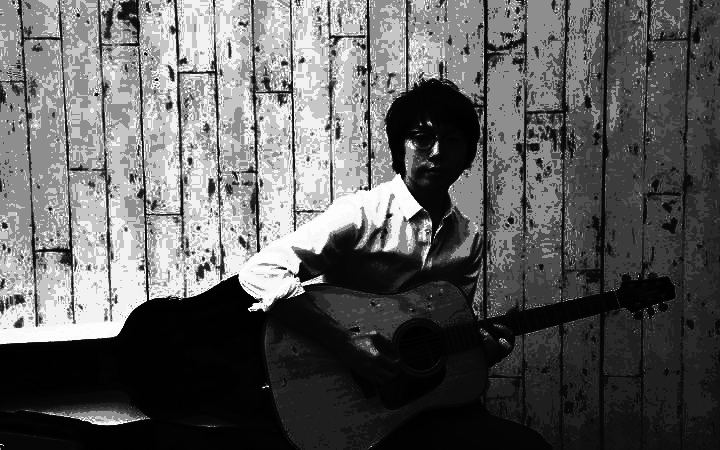
\includegraphics[width=0.4\textwidth]{yuu_cor_1.png}}
			\subfigure[直方图均衡后灰度图(p=2)]{
				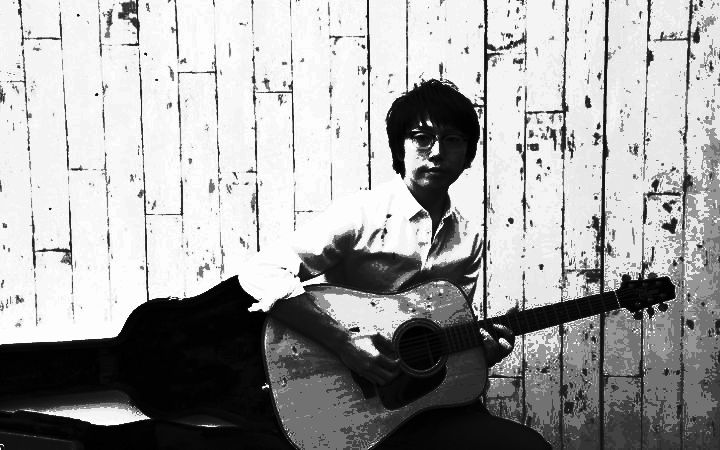
\includegraphics[width=0.4\textwidth]{yuu_cor_2.png}}
			\subfigure[直方图均衡后灰度图(p=3)]{
				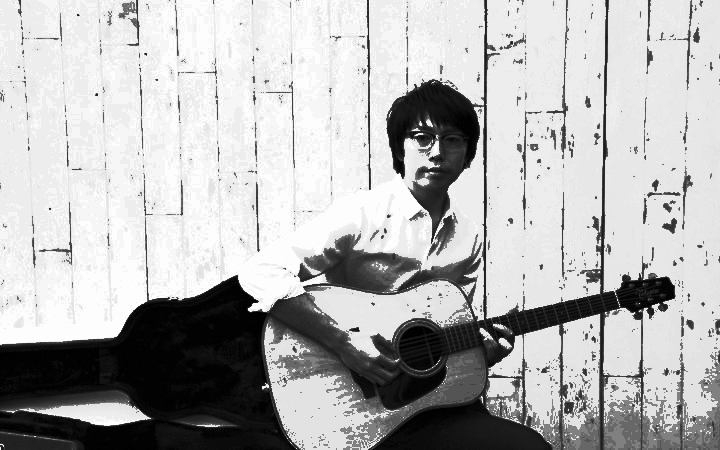
\includegraphics[width=0.4\textwidth]{yuu_cor_3.png}}
			\subfigure[直方图均衡后灰度图(p=4)]{
				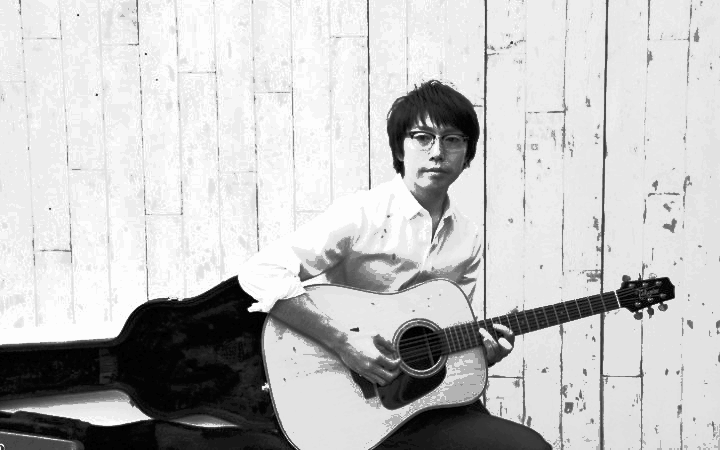
\includegraphics[width=0.4\textwidth]{yuu_cor_4.png}}
			\subfigure[直方图均衡后灰度图(p=5)]{
				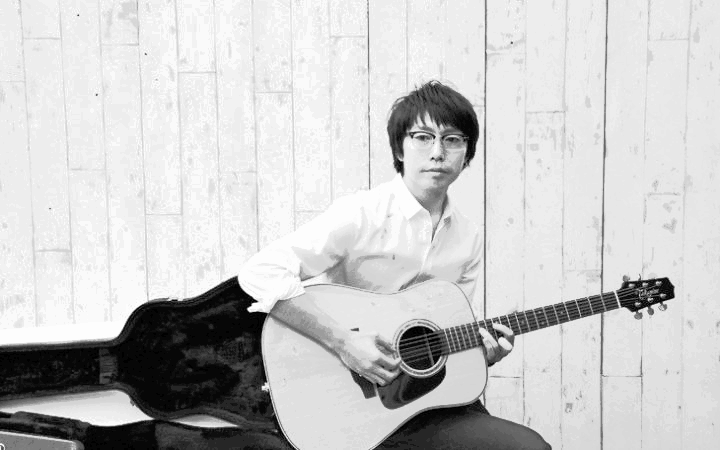
\includegraphics[width=0.4\textwidth]{yuu_cor_5.png}}
			\subfigure[原灰度图]{
				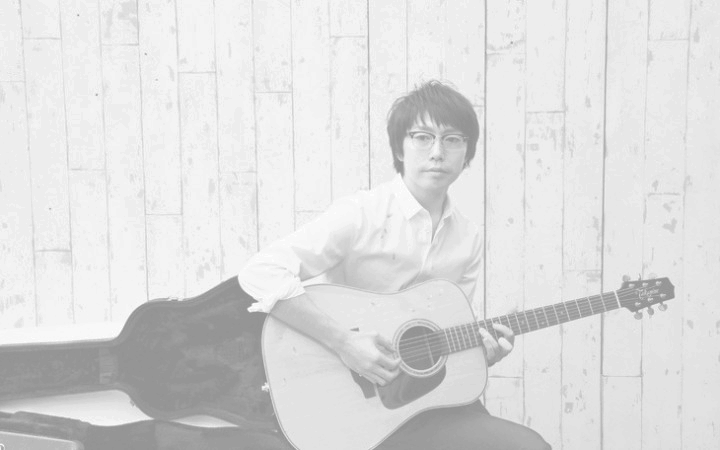
\includegraphics[width=0.4\textwidth]{yuu_grey.png}}
				\caption{图片二直方图均衡优化处理后灰度图效果}
			\end{figure}

			\begin{figure}[H]
			\centering
			\subfigure[直方图均衡后直方图(p=1)]{
				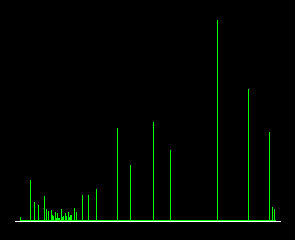
\includegraphics[width=0.4\textwidth]{yuu_cor_1_hist.png}}
			\subfigure[直方图均衡后直方图(p=2)]{
				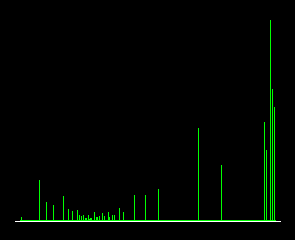
\includegraphics[width=0.4\textwidth]{yuu_cor_2_hist.png}}
			\subfigure[直方图均衡后直方图(p=3)]{
				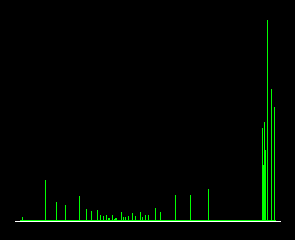
\includegraphics[width=0.4\textwidth]{yuu_cor_3_hist.png}}
			\subfigure[直方图均衡后直方图(p=4)]{
				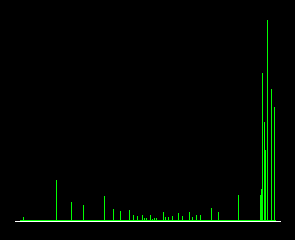
\includegraphics[width=0.4\textwidth]{yuu_cor_4_hist.png}}
			\subfigure[直方图均衡后直方图(p=5)]{
				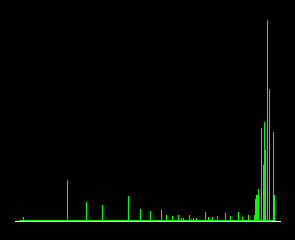
\includegraphics[width=0.4\textwidth]{yuu_cor_5_hist.png}}
			\subfigure[原直方图]{
				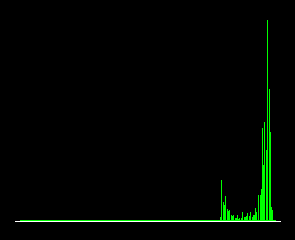
\includegraphics[width=0.4\textwidth]{yuu_grey_hist.png}}
				\caption{图片二直方图均衡优化处理后灰度分布}
			\end{figure}

			从结果可以发现,随着分段数$p$的增大,均衡后的灰度图越来越接近于原图;随着$p$的减小,均衡后的灰度图越来越接近于优化前的均衡灰度图($p=1$)。就效果而言,取$p=4$与$p=5$的均衡灰度图效果优于前三幅,说明这种优化是合理的。\newline

			\begin{figure}[H]
			\centering
			\subfigure[直方图均衡后灰度图(p=1)]{
				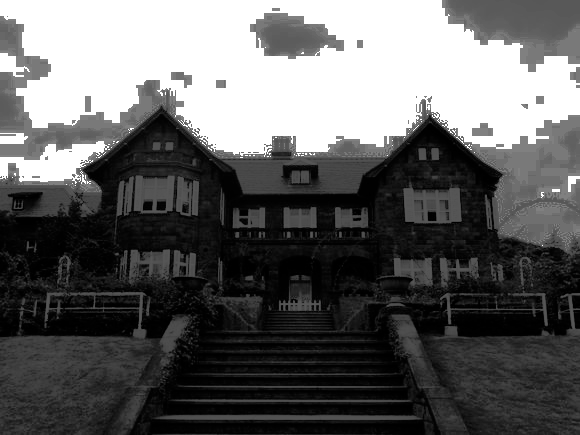
\includegraphics[width=0.4\textwidth]{rokkenjima_cor_1.png}}
			\subfigure[直方图均衡后灰度图(p=2)]{
				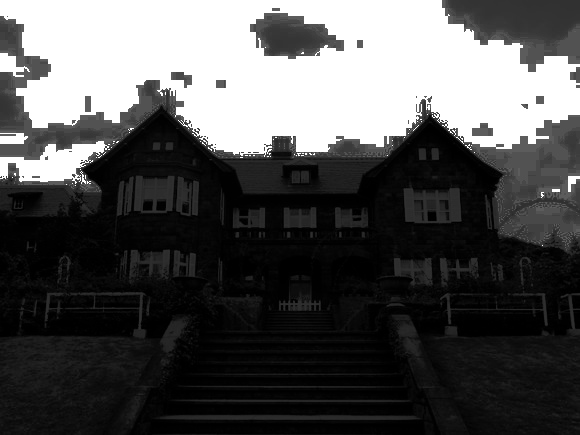
\includegraphics[width=0.4\textwidth]{rokkenjima_cor_2.png}}
			\subfigure[直方图均衡后灰度图(p=3)]{
				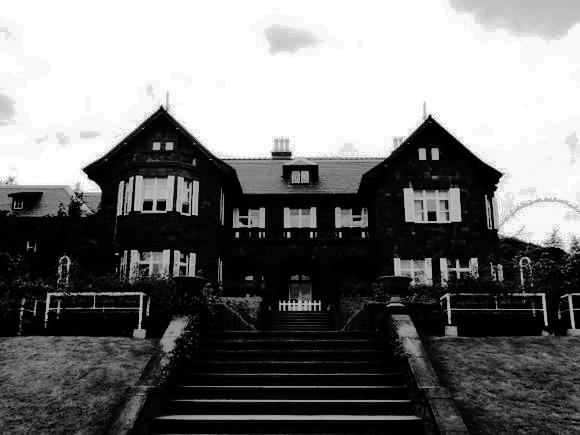
\includegraphics[width=0.4\textwidth]{rokkenjima_cor_3.png}}
			\subfigure[直方图均衡后灰度图(p=4)]{
				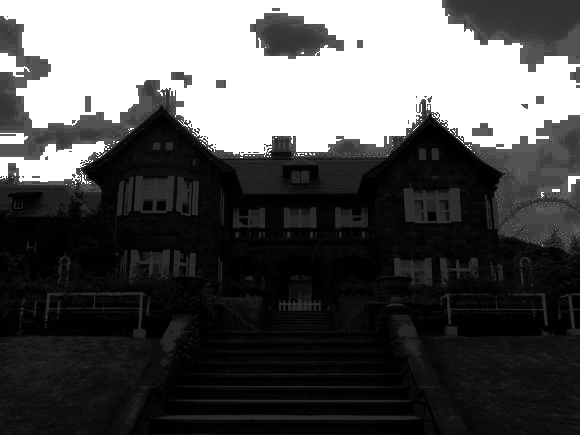
\includegraphics[width=0.4\textwidth]{rokkenjima_cor_4.png}}
			\subfigure[直方图均衡后灰度图(p=5)]{
				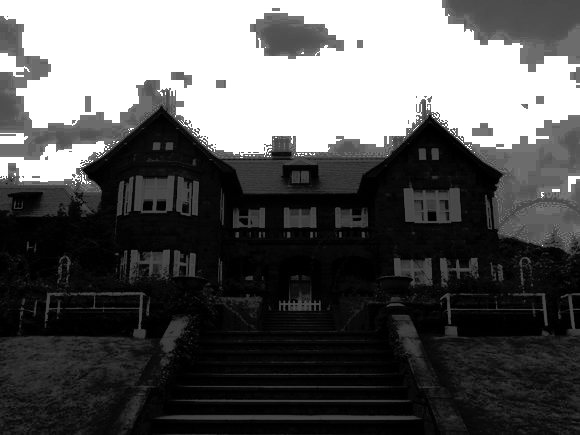
\includegraphics[width=0.4\textwidth]{rokkenjima_cor_5.png}}
			\subfigure[原灰度图]{
				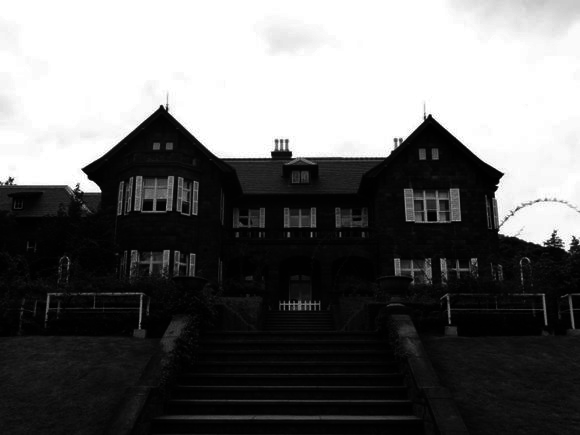
\includegraphics[width=0.4\textwidth]{rokkenjima_grey.png}}
				\caption{图片三直方图均衡优化处理后灰度图效果}
			\end{figure}


			\begin{figure}[H]
			\centering
			\subfigure[直方图均衡后直方图(p=1)]{
				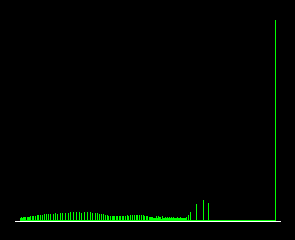
\includegraphics[width=0.4\textwidth]{rokkenjima_cor_1_hist.png}}
			\subfigure[直方图均衡后直方图(p=2)]{
				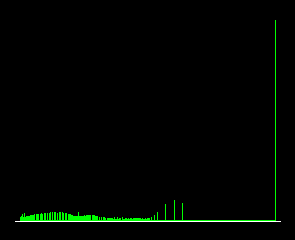
\includegraphics[width=0.4\textwidth]{rokkenjima_cor_2_hist.png}}
			\subfigure[直方图均衡后直方图(p=3)]{
				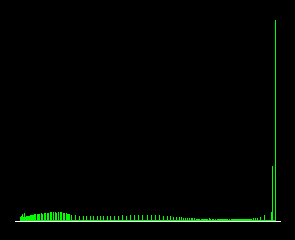
\includegraphics[width=0.4\textwidth]{rokkenjima_cor_3_hist.png}}
			\subfigure[直方图均衡后直方图(p=4)]{
				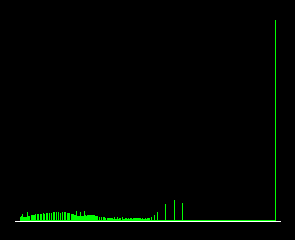
\includegraphics[width=0.4\textwidth]{rokkenjima_cor_4_hist.png}}
			\subfigure[直方图均衡后直方图(p=5)]{
				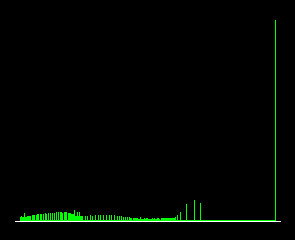
\includegraphics[width=0.4\textwidth]{rokkenjima_cor_5_hist.png}}
			\subfigure[原直方图]{
				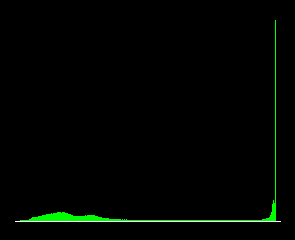
\includegraphics[width=0.4\textwidth]{rokkenjima_grey_hist.png}}
				\caption{图片三直方图均衡优化处理后灰度分布}
			\end{figure}

			但是对于图片三,上述规律并不明显,主要体现在存在一个像素数十分庞大的灰度级255,由于灰度级是离散的,整体的均衡性导致了灰度级断层的出现,从而无法呈现出较浅的像素。但是这里取$p=3$呈现出的效果仍然自然,说明在这种情况下,合适的段数$p$仍可以优化均衡的效果。\newline

			
			\indent但这并不代表着对于所有图片,取$p=4$与$p=5$结果都为最好,比如在用图片一进行分段的时候,发现还是取$p=1$即不优化的效果最好,说明$p$的最终取值还要由不同图片的性质决定。

		\subsection{总结}
			两种图片结果的比较,使我们发现直方图均衡并不是万能的。经分析,优化前的算法不适合处理小主体图片,因为如果这样,和主体无关的部分(比如背景)覆盖的灰度就会成为图片的主要灰度,在均衡的时候,主要灰度的扩散会严重影响主体相关的灰度,导致背景细节被突出,主体细节被减弱。优化后的算法试图将较深和较浅的灰度分隔开,一定程度上保护了主体相关的灰度,对部分图片可以达到更好的效果。\newline

			\indent同时,直方图均衡并不适合某种灰度级数量过多的情况,因为这样可能会导致灰度的断层,导致画面不够均匀。


	\section{任务二:灰度线性拉伸(压缩)}
		\subsection{算法实现}
		将灰度图像$f(x,y)$中$[a,b]$的灰度范围变化为$[c,d]$,有两种处理方式。\newline
		\indent若要使得变换后所有灰度都处于$[c,d]$内,则变换函数$T_l$可以表示为
		\[
		g(x,y)=\left\{
		\begin{array}{lcl}
		c & & ,{0 <= f(x,y) < a} \\
		\frac{d-c}{b-a} * (f(x,y)-a) + c & & ,{a \leq f(x,y) \leq b} \\
		d & & ,{b < f(x,y) <= 255} \\
		\end{array}\right.
		\]
		\indent若要使得变换后整体灰度范围不变,则可以采用分段线性变换。假设原图灰度范围为$[Y_{min},Y_{max}]$则变换函数$T_{pl}$可以表示为
		\[
		g(x,y)=\left\{
		\begin{array}{lcl}
		\frac{c-Y_{min}}{a-Y_{min}} * (f(x,y)-Y_{min}) + Y_{min} & & ,{Y_{min} <= f(x,y) < a} \\
		\frac{d-c}{b-a} * (f(x,y)-a) + c & & ,{a \leq f(x,y) \leq b} \\
		\frac{Y_{max}-d}{Y_{max}-b} * (f(x,y)-b) + d & & ,{b < f(x,y) <= Y_{max}} \\
		\end{array}\right.
		\]


		\subsection{处理效果}
			\subsubsection{局部线性拉伸}
			\begin{figure}[H]
			\centering
			\subfigure[改变范围拉伸后灰度图]{
				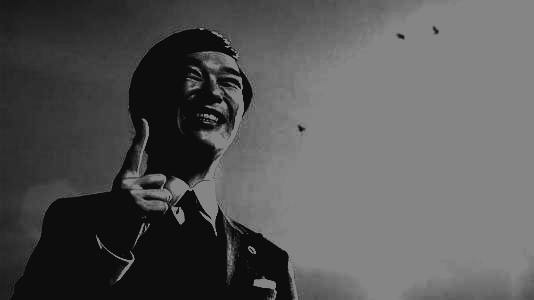
\includegraphics[width=0.4\textwidth]{lh_str_local.png}}
			\subfigure[改变范围拉伸后直方图]{
				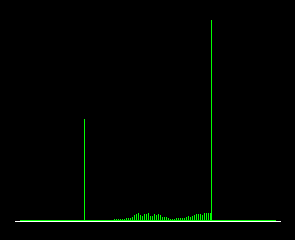
\includegraphics[width=0.4\textwidth]{lh_str_local_hist.png}}
			\subfigure[不改变范围拉伸后灰度图]{
				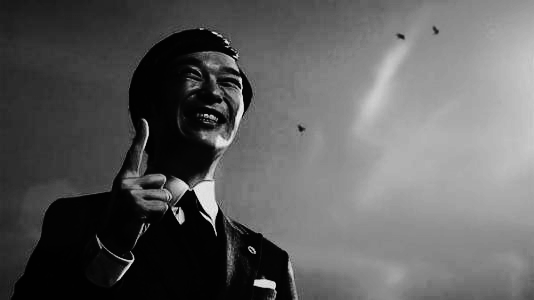
\includegraphics[width=0.4\textwidth]{lh_str_piece.png}}
			\subfigure[不改变范围拉伸后直方图]{
				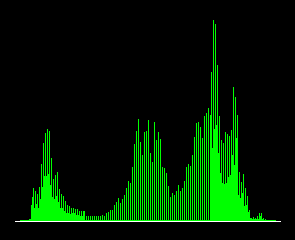
\includegraphics[width=0.4\textwidth]{lh_str_piece_hist.png}}
			\subfigure[原灰度图]{
				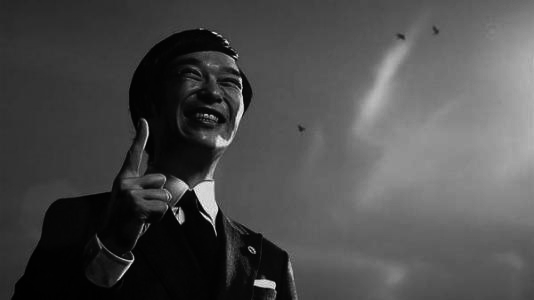
\includegraphics[width=0.4\textwidth]{lh_grey.png}}
			\subfigure[原直方图]{
				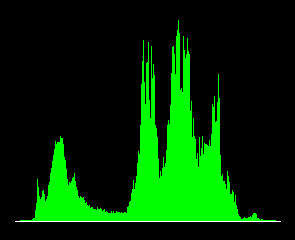
\includegraphics[width=0.4\textwidth]{lh_grey_hist.png}}
				\caption{局部线性拉伸效果}
			\end{figure}

			该实例为将原灰度图$[96,159]$范围的灰度级拉伸至$[64,191]$范围的结果。

			\subsubsection{全局线性拉伸}
			\begin{figure}[H]
			\centering
			\subfigure[线性拉伸后灰度图]{
				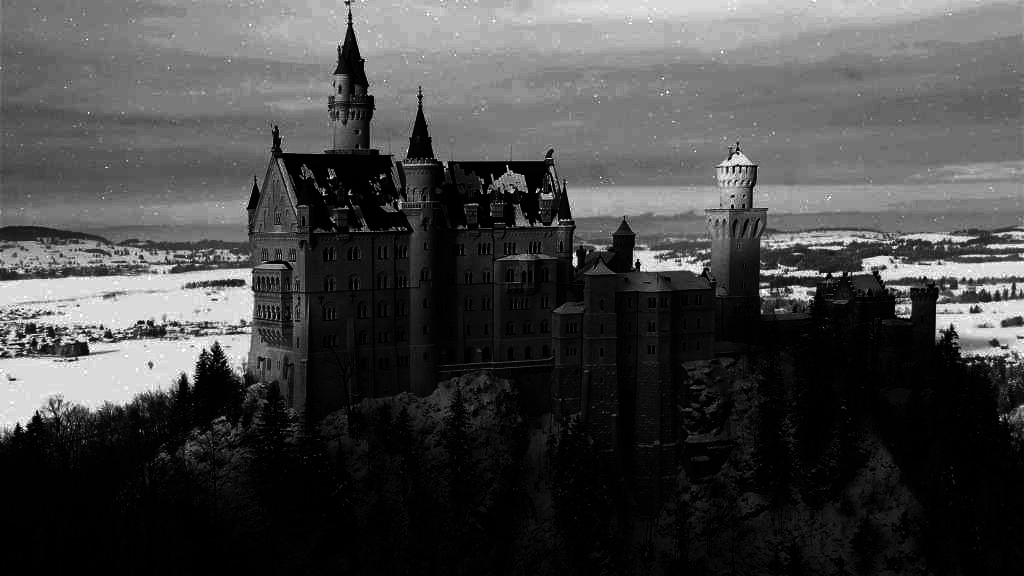
\includegraphics[width=0.4\textwidth]{cas_str_local.png}}
			\subfigure[线性拉伸后直方图]{
				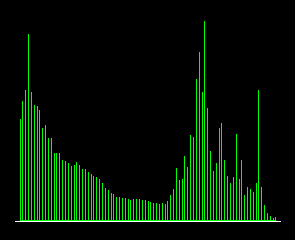
\includegraphics[width=0.4\textwidth]{cas_str_local_hist.png}}
			\subfigure[直方图均衡后灰度图]{
				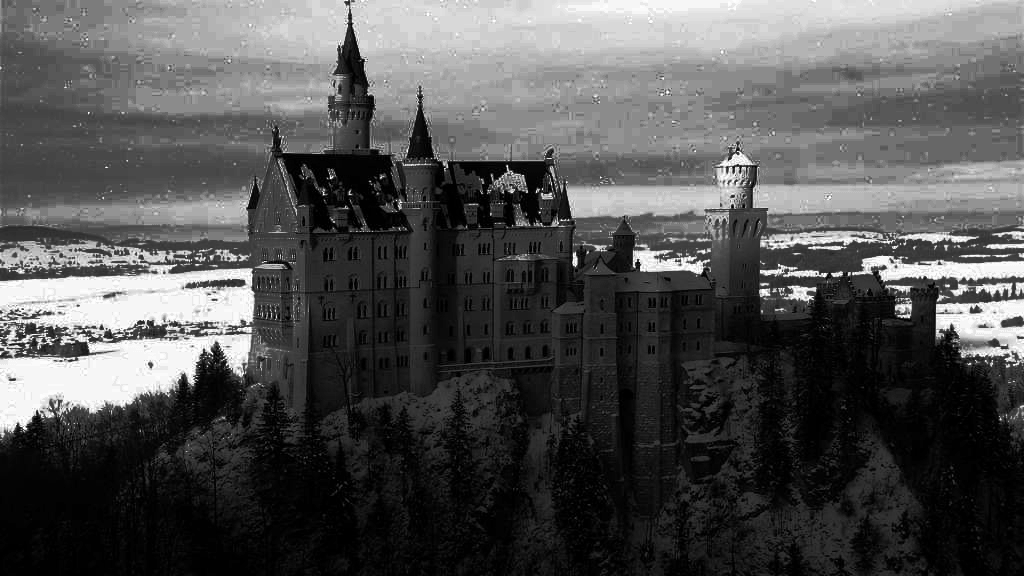
\includegraphics[width=0.4\textwidth]{cas_cor_1.png}}
			\subfigure[直方图均衡后灰度图]{
				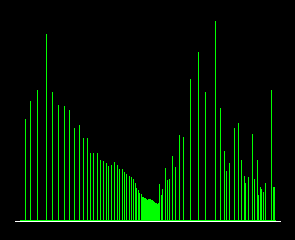
\includegraphics[width=0.4\textwidth]{cas_cor_1_hist.png}}
			\subfigure[原灰度图]{
				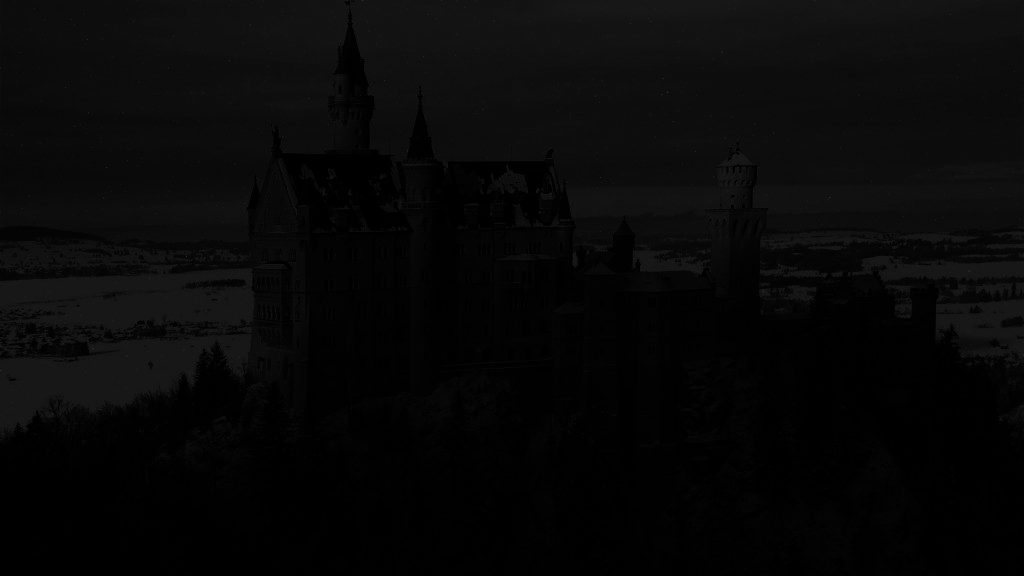
\includegraphics[width=0.4\textwidth]{cas_grey.png}}
			\subfigure[原直方图]{
				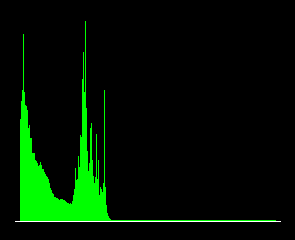
\includegraphics[width=0.4\textwidth]{cas_grey_hist.png}}
			\caption{线性拉伸与直方图均衡效果对比}
			\end{figure}
			该实例为将原灰度图灰度范围拉伸至$[0,255]$范围的结果,直方图均衡分段数$p=1$。
		\subsection{总结}
		灰度线性调整可以自由地对某一区域灰度进行拉伸或压缩,有选择性地突出或抑制灰度区间,较为灵活。但是全局线性拉伸呈现出的效果不如直方图均衡清晰,说明灰度线性调整不适合于挖掘图像细节。
\end{document}

